
\section{Architecture Integration}

\subsection{Model Support}

\begin{table}[H]
\centering
\small
\begin{tabular}{llllll}
\toprule
\textbf{Architecture} & \textbf{Class} & \textbf{Nested?} & \textbf{RoPE?} & \textbf{GQA?} & \textbf{Verified} \\
\midrule
DistilBERT & \texttt{MultiHeadSelfAttention} & No & No & No &  \\
RoBERTa & \texttt{BertSelfAttention} & Yes & No & No & 0.85 \\
GPT-2 & \texttt{GPT2Attention} (Conv1D) & No & No & No & 0.85 \\
Qwen3.5 & \texttt{Qwen3Attention} & No & Yes & Yes & 0.85 \\
\bottomrule
\end{tabular}
\end{table}

\subsection{Weight Transfer}

The \texttt{copy\_weights} method handles three patterns:

\subsubsection{GPT-2 (Fused Conv1D)}

\begin{lstlisting}
if hasattr(src, "c\_attn"):
    w = src.c\_attn.weight.data
    if isinstance(src.c\_attn, Conv1D):
        w = w.t()  # (in, out) $\to$ (out, in)
    q\_w, k\_w, v\_w = w.chunk(3, dim=0)
\end{lstlisting}

\subsubsection{RoBERTa (Nested)}

\begin{lstlisting}
elif hasattr(src, "self") and hasattr(src.self, "query"):
    extracted["q"] = src.self.query.weight.data
    extracted["k"] = src.self.key.weight.data
    extracted["v"] = src.self.value.weight.data
    extracted["o"] = src.output.dense.weight.data
\end{lstlisting}

\subsubsection{DistilBERT (Flat)}

\begin{lstlisting}
else:
    extracted["q"] = src.q\_lin.weight.data
    extracted["k"] = src.k\_lin.weight.data
    extracted["v"] = src.v\_lin.weight.data
    extracted["o"] = src.out\_lin.weight.data
\end{lstlisting}

\subsection{Nested Encoder Bypass}

For RoBERTa, \texttt{out\_lin} is outside the attention. We set 
\texttt{is\_nested\_encoder = True} and skip \texttt{out\_proj} in the forward pass.

\begin{lstlisting}
if self.is\_nested\_encoder:
    return out, None
output = self.out\_proj(out)
\end{lstlisting}

For DistilBERT, \texttt{out\_lin} is inside; \texttt{is\_nested\_encoder = False}.

\subsection{GQA Support}

For Qwen3.5 with $H_{kv} < H$:

\begin{lstlisting}
if self.num\_heads != self.num\_kv\_heads:
    repeats = self.num\_heads // self.num\_kv\_heads
    k = repeat\_kv(k, repeats)
    v = repeat\_kv(v, repeats)
\end{lstlisting}

\subsection{RoPE Support}

We support partial RoPE:

\begin{lstlisting}
if position\_embeddings is not None:
    cos, sin = position\_embeddings
    q, k = apply\_rotary\_pos\_emb(q, k, cos, sin)
\end{lstlisting}

\texttt{apply\_rotary\_pos\_emb} handles cases where \texttt{rotary\_dim \textless{} head\_dim}.

\subsection{Injection Algorithm}

\textbf{Algorithm 2:} Inject RALA into a layer
\begin{lstlisting}
Input:  layer, config, old\_attn
Output: new attention module

1: new $\leftarrow$ RALALinearAttention(config, old\_attn=old\_attn)
2: if copy\_weights failed:
3:     log warning
4: if layer.attention.self:
5:     layer.attention.self $\leftarrow$ new; new.is\_nested\_encoder $\leftarrow$ True
6: elif layer.attention:
7:     layer.attention $\leftarrow$ new
8: elif layer.self\_attn:
9:     layer.self\_attn $\leftarrow$ new
10: return new
\end{lstlisting}

\subsection{Double-Injection Guard}

We check for prior injection:

\begin{lstlisting}
if isinstance(src\_attn, RALALinearAttention):
    return None
if "RALA" in src\_attn.\_\_class\_\_.\_\_name\_\_:
    return None
\end{lstlisting}

\subsection{Qwen3.5 DeltaNet Skip}

Some Qwen layers use GatedDeltaNet, which is incompatible with RALA. We 
skip these:

\begin{lstlisting}
if "DeltaNet" in c\_name or "LinearAttention" in c\_name:
    return None
\end{lstlisting}

\subsection{Failure Handling}

\begin{table}[H]
\centering
\small
\begin{tabular}{lll}
\toprule
\textbf{Failure} & \textbf{Detection} & \textbf{Response} \\
\midrule
Missing weight & \texttt{copy\_weights} logs & Random init for that proj \\
Shape mismatch & Shape check & Truncate or repeat \\
Zero norm & Norm check & Warning, continue \\
Injection exception & try/except & Return None \\
\bottomrule
\end{tabular}
\end{table}

\subsection{Compatibility Notes}

\subsubsection{Cross-Attention}

RALA does \textbf{not} support cross-attention. \texttt{encoder\_hidden\_states} is ignored.

\subsubsection{Padded Sequences}

Padding tokens are masked via \texttt{get\_token\_valid\_mask}. The prefix scan 
respects this mask: padded positions do not contribute to $S$ or $z$.

\subsubsection{Mixed Precision}

RALA runs in the base model's dtype (FP16 typically). The prefix sums are 
computed in FP16, which may lose precision for long sequences. Consider 
FP32 for $L > 512$.
\begin{lstlisting}

---
\end{lstlisting}

\begin{figure}[H]
\centering
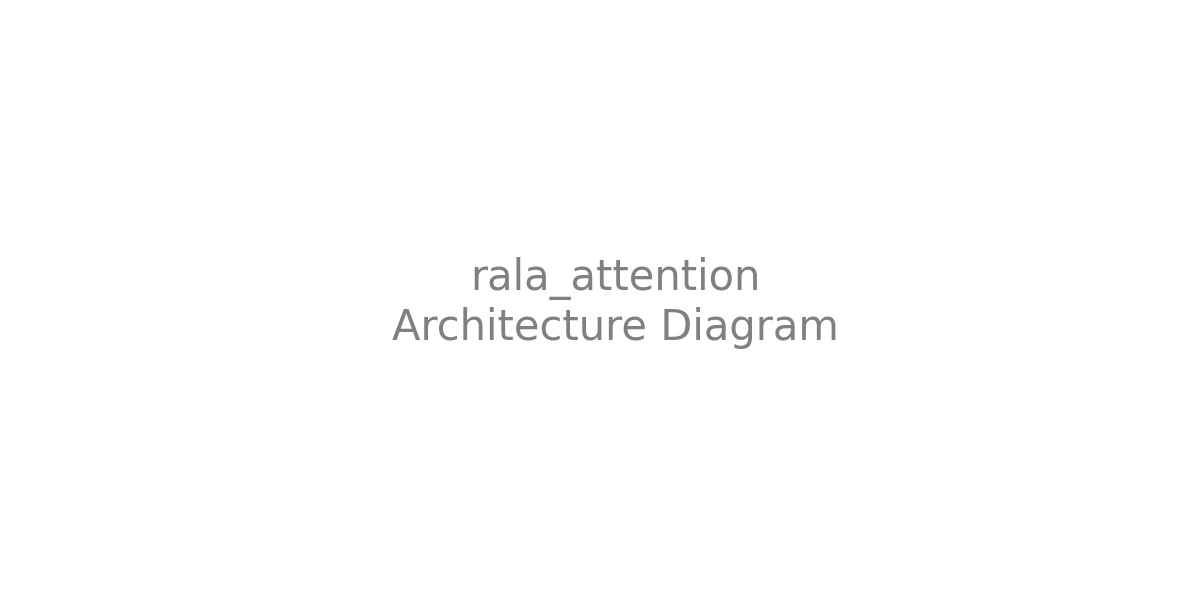
\includegraphics[width=\linewidth]{figures/architecture.png}
\caption{High-level architectural diagram of rala\_attention.}
\label{fig:arch\_rala-attention}
\end{figure}

